\documentclass[11pt]{article}
\usepackage[utf8]{inputenc}
\usepackage[T1]{fontenc}
\usepackage{amsmath}
\usepackage{amssymb} % Needed for \eth
\usepackage{graphicx}
\usepackage{geometry}
\usepackage{tikz}
\usepackage{pgfplots} % For plots
\usepackage{ulem}     % For underline, using normalem to avoid messing with \emph

\geometry{a4paper, margin=1in}
\usetikzlibrary{positioning, arrows.meta, shapes.geometric} % For TikZ diagrams
\pgfplotsset{compat=1.18} % Use a recent PGFPlots version

% Custom commands (optional)
\newcommand{\avg}[1]{\overline{#1}}
\newcommand{\prob}[1]{P(#1)}
\newcommand{\ProbDens}[1]{\mathcal{P}(#1)} % Using script P for density
\newcommand{\vect}[1]{\vec{#1}}
\newcommand{\dd}[1]{\mathrm{d}#1} % Differential d
\newcommand{\pderiv}[2]{\frac{\partial #1}{\partial #2}}
\newcommand{\deriv}[2]{\frac{\mathrm{d} #1}{\mathrm{d} #2}}
\newcommand{\muState}{\mu\text{-state}} % Microstate
\newcommand{\OmegaE}{\Omega(E)}
\newcommand{\omegaE}{\omega(E)}
\newcommand{\PhiE}{\Phi(E)}
\newcommand{\deltaE}{\delta E}
\newcommand{\ethbar}{\text{\it{đ}}} % \eth symbol for inexact differential
\newcommand{\kb}{k_B} % Boltzmann constant
\newcommand{\gasR}{R}

\title{Physics 415 - Lecture 12: Thermodynamic Potentials}
\date{February 17, 2025}
\author{} % Author not specified

\begin{document}

\maketitle
\thispagestyle{empty}

\section*{Summary} % [cite: 1]

\begin{itemize}
    \item Fundamental relation (for simple system with $V$ as external parameter): $dE = T dS - p dV$[cite: 2]. Natural variables for $E$ are $(S,V)$.
    \item First Law: $dE = \ethbar Q - \ethbar W$[cite: 2].
    \item Second Law: For a thermally isolated system, $\Delta S \ge 0$ for any spontaneous process[cite: 2]. Equilibrium corresponds to $S=\text{max}$[cite: 2].
\end{itemize}

\section*{Thermodynamic Potentials} % [cite: 3]

The thermodynamic variables include $\{E, S, T, V, p, \dots\}$[cite: 3]. (More variables exist, e.g., chemical potential $\mu$, particle number $N$, but focus on these for now).

For a closed system, we might specify $(E, V)$ as independent variables [source: 4]. Other quantities are then determined, e.g., $S=S(E,V)$, $T=T(E,V)$, $p=p(E,V)$ [source: 4].
Equivalently, we can take $(S,V)$ as independent variables, and then $E=E(S,V)$ is determined [source: 5]. From the fundamental relation $dE = T dS - p dV$, we can find $T$ and $p$ [source: 6]:
\[ T = \left( \pderiv{E}{S} \right)_V, \quad p = -\left( \pderiv{E}{V} \right)_S \text{[cite: 6]} \]
The pair $(S,V)$ are the "natural variables" for the internal energy function $E$.

In practice, we would like to use variables that are more easily controlled experimentally, like temperature $T$ and pressure $p$, as independent variables, instead of $S$ and $E$ [source: 7]. Thermodynamic potentials allow us to switch the set of independent variables while retaining all thermodynamic information.

\subsection*{Helmholtz Free Energy (F)} % [cite: 8]

Consider putting a system A (of interest) in contact with a heat bath A', which is a much larger system that fixes the temperature $T$ of system A [source: 8, 9]. The combined system A+A' is isolated, but A itself is not (it can exchange heat with A') [source: 9]. We are interested in system A at fixed $(T,V)$.

\begin{center}
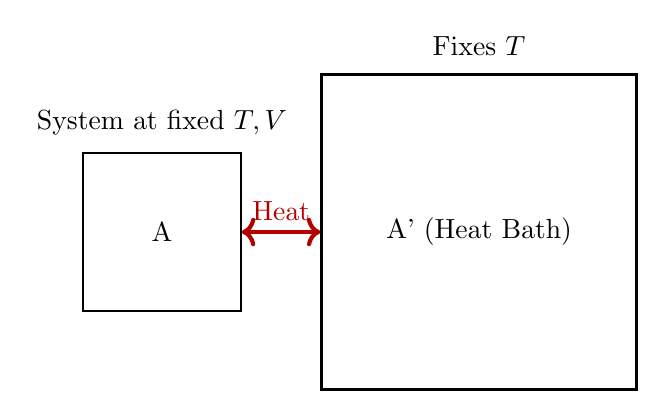
\begin{tikzpicture}
    \node (A) [draw, thick, minimum width=2cm, minimum height=2cm, label=center:A] {};
    \node (Aprime) [draw, thick, minimum width=4cm, minimum height=4cm, right=1cm of A, label=center:A' (Heat Bath)] {};
    % Interface allowing heat exchange
    \draw [line width=1.5pt, red!70!black, <->] (A.east) -- (Aprime.west) node [midway, above] {Heat};
    % Labels
    \node at (A.north) [above=0.1cm] {System at fixed $T, V$};
    \node at (Aprime.north) [above=0.1cm] {Fixes $T$};
\end{tikzpicture}
\end{center}

What is the work done *by* system A? From the first law $dE = \ethbar Q - \ethbar W$, we have $\ethbar W = \ethbar Q - dE$[cite: 10].
For a quasi-static process occurring at constant temperature $T$, the heat absorbed by A is $\ethbar Q = T dS$ [cite: 11] (where $S$ is the entropy of system A).
\[ \implies \ethbar W = T dS - dE \text{[cite: 11]} \]
Since $T$ is constant, $T dS = d(TS)$[cite: 11].
\[ \ethbar W = d(TS) - dE = - d(E - TS) \text{[cite: 11]} \]
We define the \textbf{Helmholtz Free Energy} $F$[cite: 11]:
\[ F \equiv E - TS \text{[cite: 11]} \]
Then, for a quasi-static, isothermal process[cite: 11]:
\[ \ethbar W = -dF \text{[cite: 11]} \]
The infinitesimal work done by the system equals the decrease in its Helmholtz free energy[cite: 12].
For a finite process from state $i$ to $f$: $W_{if} = -\Delta F = F_i - F_f$.

$F$ is a function of state[cite: 12]. What are its natural variables?
$dF = dE - d(TS) = dE - T dS - S dT$[cite: 14].
Substitute the fundamental relation $dE = T dS - p dV$[cite: 14]:
\[ dF = (T dS - p dV) - T dS - S dT \]
\[ \implies dF = -S dT - p dV \text{[cite: 14]} \]
This shows that the natural variables for $F$ are $(T, V)$[cite: 14]. $F = F(T,V)$.
From this differential form, we can find $S$ and $p$[cite: 14]:
\[ S = - \left( \pderiv{F}{T} \right)_V, \quad p = - \left( \pderiv{F}{V} \right)_T \text{[cite: 14]} \]
Knowing $F(T,V)$ allows us to find $S$ and $p$[cite: 14]. We can also find $E$[cite: 15]:
\[ E = F + TS = F - T \left( \pderiv{F}{T} \right)_V \text{[cite: 15]} \]
This can also be written using a "Gibbs-Helmholtz" type relation[cite: 15]:
\[ E = -T^2 \left( \pderiv{}{T} \frac{F}{T} \right)_V \text{[cite: 15]} \]

The mathematical procedure used to pass from $E(S,V)$ to $F(T,V)$ is called a \textbf{Legendre Transform}[cite: 16].
We started with $E(S,V)$ and $T = (\partial E / \partial S)_V$[cite: 16].
We defined $F = E - TS$[cite: 16]. The new function $F$ depends on $T$ instead of $S$.
This is analogous to passing from the Lagrangian $L(q, \dot{q})$ to the Hamiltonian $H(q,p)$ in classical mechanics, where $p = \partial L / \partial \dot{q}$[cite: 17]:
$H(q,p) = p \dot{q} - L(q, \dot{q})$[cite: 17].
(Analogy: $S \leftrightarrow \dot{q}$, $T \leftrightarrow p$, $E \leftrightarrow L$, $F \leftrightarrow -H$)[cite: 17].

\subsection*{Enthalpy (H)} % [cite: 17]

Just as we considered a system at fixed (controllable) $T$, we may consider a system maintained at fixed pressure $p$ (e.g., open to atmosphere, or piston with constant external force)[cite: 17].

For a system at fixed $V$, heat absorbed is $\ethbar Q_V = dE_V$[cite: 18].
For a system undergoing a quasi-static process at fixed $p$[cite: 18]:
\[ \ethbar Q |_p = dE |_p + \ethbar W |_p = dE |_p + p dV |_p \text{[cite: 18]} \]
Since $p$ is constant, $p dV|_p = d(pV)|_p$[cite: 19].
\[ \ethbar Q |_p = dE |_p + d(pV) |_p = d(E+pV)|_p \text{[cite: 19]} \]
We define the \textbf{Enthalpy} $H$[cite: 19]:
\[ H \equiv E + pV \text{[cite: 19]} \]
Then, for a quasi-static process at constant pressure[cite: 19]:
\[ \ethbar Q |_p = dH |_p \text{[cite: 19]} \]
The heat absorbed at constant pressure equals the change in enthalpy[cite: 19].
$H$ is a function of state[cite: 20]. What are its natural variables?
\[ dH = dE + d(pV) = dE + p dV + V dp \text{[cite: 21]} \]
Substitute $dE = T dS - p dV$[cite: 21]:
\[ dH = (T dS - p dV) + p dV + V dp \]
\[ \implies dH = T dS + V dp \text{[cite: 21]} \]
The natural variables for $H$ are $(S, p)$[cite: 20]. $H=H(S,p)$.
From this, we can find $T$ and $V$[cite: 21]:
\[ T = \left( \pderiv{H}{S} \right)_p, \quad V = \left( \pderiv{H}{p} \right)_S \text{[cite: 21]} \]
If a process occurs at constant pressure and is thermally isolated ($\ethbar Q=0$), then $dH=0$[cite: 21]. Enthalpy is conserved in such processes[cite: 22].

The heat capacity at constant pressure $C_p$[cite: 22]:
$\ethbar Q|_p = C_p dT$[cite: 22]. Since $\ethbar Q|_p = dH|_p$:
\[ dH|_p = C_p dT \text{[cite: 22]} \]
Considering $H=H(T,p)$, $dH = (\partial H / \partial T)_p dT + (\partial H / \partial p)_T dp$.
At constant $p$, $dH|_p = (\partial H / \partial T)_p dT$.
\[ \implies C_p = \left( \pderiv{H}{T} \right)_p \text{[cite: 22]} \]
(Compare with $C_V = (\partial E / \partial T)_V$)[cite: 22].

\textbf{Example:} Monatomic ideal gas[cite: 22].
$E = \frac{3}{2}NT$ and $pV = NT$[cite: 23]. (Using $T$ in energy units).
$H = E + pV = \frac{3}{2} NT + NT = \frac{5}{2} NT$[cite: 23].
$C_p = (\partial H / \partial T)_p = \frac{5}{2} N$[cite: 23].
In molar terms (with $T$ in Kelvin): $E = \frac{3}{2} \nu \gasR T$, $pV = \nu \gasR T$.
$H = E + pV = \frac{3}{2} \nu \gasR T + \nu \gasR T = \frac{5}{2} \nu \gasR T$.
$C_p = (\partial H / \partial T)_p = \frac{5}{2} \nu \gasR$.
Molar specific heat $c_p = C_p/\nu = \frac{5}{2} \gasR$. Matches $c_p = c_v + R = \frac{3}{2}\gasR + \gasR = \frac{5}{2}\gasR$[cite: 23]. $\checkmark$

\subsection*{Gibbs Free Energy (G)} % [cite: 24]

To describe a system at constant (externally specified) $T$ and $p$, we use the \textbf{Gibbs Free Energy} $G$[cite: 24]:
\[ G \equiv E - TS + pV = F + pV = H - TS \text{[cite: 24]} \]
$G$ is a state function [source: 24]. What are its natural variables?
$dG = dH - d(TS) = dH - T dS - S dT$ [source: 24].
Substitute $dH = T dS + V dp$ [source: 24]:
\[ dG = (T dS + V dp) - T dS - S dT \]
\[ \implies dG = -S dT + V dp \text{[cite: 25]} \]
The natural variables for $G$ are $(T, p)$[cite: 24]. $G=G(T,p)$.
From this, we can find $S$ and $V$[cite: 25]:
\[ S = - \left( \pderiv{G}{T} \right)_p, \quad V = \left( \pderiv{G}{p} \right)_T \text{[cite: 25]} \]
We can also find $H$[cite: 25]:
\[ H = G + TS = G - T \left( \pderiv{G}{T} \right)_p \text{[cite: 25]} \]
This can also be written as[cite: 25]:
\[ H = -T^2 \left( \pderiv{}{T} \frac{G}{T} \right)_p \text{[cite: 25]} \]

\section*{Summary of Potentials}

The functions $E, F, H, G$ are called "thermodynamic potentials"[cite: 26].
\begin{itemize}
    \item Internal Energy: $E(S,V) \implies dE = T dS - p dV$
    \item Helmholtz Free Energy: $F(T,V) = E-TS \implies dF = -S dT - p dV$
    \item Enthalpy: $H(S,p) = E+pV \implies dH = T dS + V dp$
    \item Gibbs Free Energy: $G(T,p) = E-TS+pV \implies dG = -S dT + V dp$
\end{itemize}
From any one of these potentials, expressed as a function of its natural variables, we can obtain all other thermodynamic quantities ($S, T, p, V$) by taking appropriate partial derivatives[cite: 25].

Thermodynamic potentials are also important because they are minimized in equilibrium under certain conditions (analogous to $S$ being maximized for an isolated system)[cite: 27].
\begin{itemize}
    \item For closed system at fixed $(T,V)$: $F$ is minimized in equilibrium.
    \item For closed system at fixed $(T,p)$: $G$ is minimized in equilibrium.
\end{itemize}
(To be shown later)[cite: 27]. This tells us how systems approach equilibrium when they can exchange heat with, or do work on, their environments under these specific constraints[cite: 29].

\end{document}